\documentclass{article}
\usepackage[utf8]{inputenc}
\usepackage[russian]{babel}
\usepackage[14pt]{extsizes}
\usepackage[a4paper, total={170mm,257mm},left=20mm, top=20mm]{geometry}
\pagestyle{empty}
\usepackage{mathtools}
\usepackage{caption}
\usepackage{tikz} 
\usepackage{graphicx}
\usepackage{wrapfig}
\graphicspath{{pictures/}}
\usepackage{fancyhdr}
\usepackage{float}
\usepackage{pgfplots}

\begin{document}
\begin{center}
\textbf{\Large{Федеральное государственное автономное образовательное учреждение высшего образования национальный исследовательский 
университет ИТМО}}
\end{center} \textbf{\\ \\}
\textbf{\\ \\ \\ \\ \\ \\}

\begin{center}
\LARGE\textbf{
Расчетно графическая работа по теме \\
"Производная и дифференциал"
}
\end{center}
\textbf{\\ \\ \\ \\ \\ \\ \\}

\begin{flushright}
\LARGE\textbf{Студент:}\\
\LARGE\text{Нодири Хисравхон}\\
\LARGE\textbf{группа: P3133}\\
\end{flushright}
\textbf{\\ \\ \\ \\ \\ \\}

\begin{center}
    \Large\textbf{Санкт-Петербург,} \\
    \Large\textbf{2022}
\end{center}
\newpage
\setcounter{page}{1}
\pagestyle{plain}

\centering

\LARGE\textbf{2. Наибольшее и наименьшее значения функции}
\linebreak

\large\textbf{
Из куска металла, ограниченного линиями , , требуется
выпилить деталь прямоугольной формы с наибольшей площадью.
}
\linebreak

\large{
2.1) Составьте математическую модель задачи: введите обозначения, выпишите данные, составьте уравнение (систему уравнений), содержащее неизвестное.
}
\linebreak

$$\{y = x, y = 0, x = 12\}$$
\linebreak

\large{2.2) Решите задачу аналитически, применяя необходимое и достаточное условия экстремума.}
\linebreak

\begin{center}

$S = t(12 - t) = 12t - 12^2$
\\
$S = 12 - 2t = 0$
\\
$t = 6 \Rightarrow S = t(12 - t) = 6 * 6 = 36$

\end{center}

\newpage

\large{2.3) Сделайте графическую иллюстрацию к решению задачи. Сверьтесь с аналитическим
решением.}
\linebreak


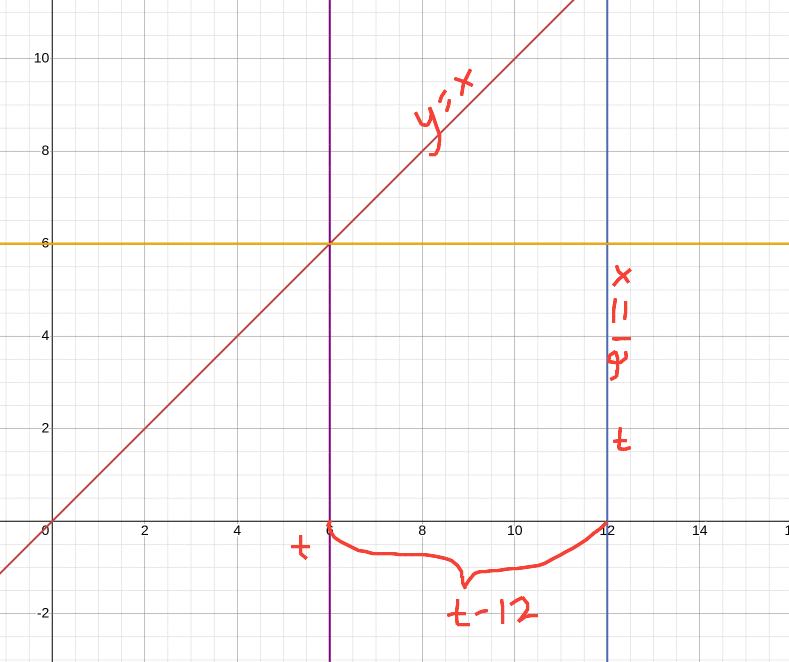
\includegraphics[scale=0.45]{pic1.png}
\linebreak

\large{2.4) Запишите ответ.}
\linebreak

Ответ: 36
\linebreak

\LARGE\textbf{3. Исследование функции}
\linebreak\linebreak
\Large{Даны функции f(x) и g(x). Проведите поочерёдно их полные исследования:}
\linebreak\linebreak
\large{3.1) Найдите область определения функции.}
$$f(x) = \frac{x + 1}{x^2 + 2x - 3} ; g(x) = \sqrt[\leftroot{5} \uproot{3} 3]{1 - cos(x)} $$

\newpage

$$f(x) = \frac{x + 1}{(x - 1)(x+3)} \Rightarrow (x - 1)(x + 3) \neq 0 ; x \in (-\infty ; +\infty)$$
$$x_1 = 1 ; x_2 = -3 ; x \neq 1, -3$$
\large{3.2) Проверьте, является ли функция чётной (нечётной), а также периодической, и укажите, как
эти свойства влияют на вид графика функции.}
$$f(-x) = \frac{-x + 1}{(-x)^2 + 2(-x) - 3}$$
$$f(-x) = \frac{1 - x}{x^2 - 2x - 3}; f(x) \neq f(-x), f(x) \neq -f(x)$$
$$g(x) = \sqrt[\leftroot{3} \uproot{3} 3]{1 - cos(x)} ; g(-x) = \sqrt[\leftroot{3} \uproot{3} 3]{1 - cos(x)}$$
$$g(x) = g(-x) \Rightarrow $$ Фун. чётная т.к $cos(x)$ период., то и $g(x)$ периодична.
$$g(x) = \sqrt[\leftroot{5} \uproot{3} 3]{1 - cos(x)} = 0$$
$$f(x) = \frac{x + 1}{(x - 1)(x + 3)} = 0$$
$$cos(x) = 1 ; x = 2 \pi k$$
$$g(x) \geq 0 ; \forall x \in (-\infty ; +\infty)$$
\large{3.3) Проверьте, является ли функция чётной (нечётной), а также периодической, и укажите, как
эти свойства влияют на вид графика функции.}
$$f(x) = \frac{x + 1}{(x - 1)(x + 3) = 0}$$
$$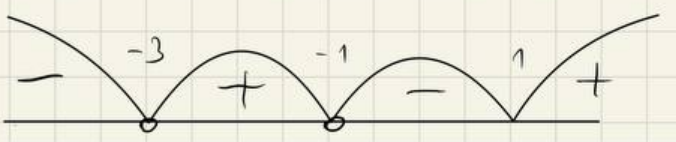
\includegraphics[scale=0.45]{pic2.png}$$
\newpage
\large{3.4) Исследуйте функцию с помощью первой производной: найдите интервалы монотонности и
экстремумы функции.}
$$f^\prime (x) = \frac{-x^2 - 2x - 5}{(x^2 + 2x - 3)^3}$$
\centering $f^\prime (x) = 0 ; x \notin R \Rightarrow $ Фун. монотонная
$$g^\prime (x) = \frac{sin(x)}{3 \sqrt[\leftroot{3} \uproot{3} 3]{(1 - cos(x)^2}} $$
$$\frac{sin(x)}{3 \sqrt[\leftroot{3} \uproot{3} 3]{(1 - cos(x))^2}} = 0$$
$$x = \pi + 2\pi k$$
$$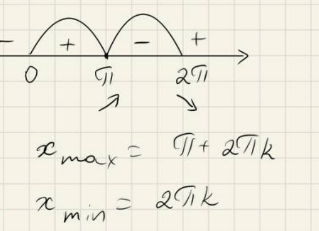
\includegraphics[scale=0.45]{pic3.png}$$
\large{3.5) Исследуйте функцию с помощью второй производной: найдите интервалы выпуклости
(вогнутости) и точки перегиба функции.}
$$f''(x) = \frac{2 * (x^2 + 2x - 3) - (x + 1)(2x + 2)}{(x^2 + 2x - 3)^2} = \frac{4x + 2}{(x^2 + 2x - 3)^2}$$
\small{Чтобы найти точки перегиба функции, нужно решить уравнение f(x) = 0. Это уравнение имеет решение x = -1/2. Следовательно, функция f(x) имеет одну точку перегиба при x = -1/2.\linebreak\linebreakЧтобы найти интервалы выпуклости (вогнутости) функции f(x), нужно определить значение f''(x) в этой точке. Подставив x = -1/2 в уравнение для f''(x), получим f''(-1/2) = -1/16. Следовательно, функция f(x) при x = -1/2 имеет выпуклый (вогнутый) характер.\linebreak\linebreakЧтобы найти интервалы выпуклости (вогнутости) функции f(x), нужно проверить значение f''(x) в других точках. Если f''(x) > 0, то функция f(x) выпуклая. Если f''(x) < 0, то функция f(x) вогнутая. Если f''(x) = 0, то функция f(x) не является ни выпуклой, ни вогнутой.}

\newpage
\large
$$g''(x) = \frac{-sin(x)}{3} \sqrt[\leftroot{3} \uproot{3} 3]{(1 - cos(x))^2}$$
\small{Чтобы найти точки перегиба функции, нужно решить уравнение g''(x) = 0. Это уравнение не имеет вещественных решений, поэтому функция g(x) не имеет точек перегиба.
}
\linebreak
\linebreak
\small{
Чтобы найти интервалы выпуклости (вогнутости) функции g(x), нужно проверить значение g''(x) в разных точках. Если g''(x) > 0, то функция g(x) выпуклая. Если g''(x) < 0, то функция g(x) вогнутая. Если g''(x) = 0, то функция g(x) не является ни выпуклой, ни вогнутой.}

\large

\large{3.6) Проверьте наличие вертикальных, горизонтальных и наклонных асимптот графика функции.}
\linebreak
\linebreak
\small
Чтобы найти вертикальные асимптоты рациональной функции, нужно найти значения x, при которых знаменатель функции равен нулю, а числитель не равен нулю. Для первой функции, f(x), знаменатель равен x\^2 + 2x - 3, поэтому вертикальные асимптоты находятся при x = -3 и x = 1.
\linebreak
\linebreak
Чтобы найти горизонтальные асимптоты рациональной функции, нужно посмотреть на ведущие члены числителя и знаменателя. Если степень числителя меньше степени знаменателя, то горизонтальной асимптотой является y = 0. Если степень числителя больше степени знаменателя, то горизонтальной асимптоты нет. Если степень числителя равна степени знаменателя, то горизонтальной асимптотой является отношение ведущих коэффициентов числителя и знаменателя. В случае f(x) степень числителя равна 1, а степень знаменателя - 2, поэтому горизонтальная асимптота равна y = 0.
\linebreak
\linebreak
Чтобы найти наклонные асимптоты рациональной функции, нужно найти ведущие члены числителя и знаменателя и разделить их. Если степень числителя меньше степени знаменателя, то наклонной асимптоты нет. Если степень числителя больше степени знаменателя, то наклонная асимптота является уравнением прямой вида y = mx + b, где m - отношение ведущих коэффициентов числителя и знаменателя, а b - y-пересечение. Если степень числителя равна степени знаменателя, нужно разделить многочлены и посмотреть на полученный коэффициент. Если коэффициент является многочленом, то наклонная асимптота - это уравнение линии, заданной главным членом коэффициента. Если коэффициент не является многочленом, то косой асимптоты не существует. В случае f(x) степень числителя равна 1, а степень знаменателя - 2, поэтому косой асимптоты нет.

\newpage

\large{3.7) Найдите точки пересечения графика с координатными осями и (при необходимости) найдите
значения функции в некоторых дополнительных точках.}
\linebreak
\linebreak
\small
Для первой функции f(x) мы можем найти точки пересечения с координатными осями, задав значение x равным 0 или значение функции равным 0.
\linebreak
\linebreak
Задание x = 0 дает нам f(0) = (0 + 1) / (0\^2 + 2*0 - 3) = 1/-3, которая не пересекает ось x.
\linebreak
\linebreak
Уравнение f(x) = 0 дает нам (x + 1) / (x\^2 + 2x - 3) = 0. Умножение обеих сторон уравнения на (x\^2 + 2x - 3) дает нам x + 1 = 0, поэтому x = -1. Это пересекает ось y в точке (0, -1).
\linebreak
\linebreak
Чтобы найти значения функции в некоторых дополнительных точках, мы можем подставить эти значения вместо x в уравнение для f(x). Например, f(1) = (1 + 1) / (1\^2 + 2*1 - 3) = 2 / 0, что является неопределенным.
\linebreak
\linebreak
Для второй функции g(x) мы можем найти точки пересечения с координатными осями аналогичным образом. Задавая x = 0, мы получаем g(0) = ∛(1 - cos(0)) = ∛(1 - 1) = ∛(0) = 0, которая пересекает ось x в точке (0, 0).
\linebreak
\linebreak
Задавая g(x) = 0, получаем ∛(1 - cos(x)) = 0, что означает, что 1 - cos(x) = 0. Решение для x дает нам x = 2pi/3 и x = 4pi/3. Они пересекают ось y в точках (2pi/3, 0) и (4pi/3, 0).
\newpage
\newpage
\newpage
\end{document}
